%!TEX program = lualatex
\documentclass[format=draft,language=chinese,category=academic-report]{hustreport}
\usepackage{booktabs}
%\usepackage [english]{babel}
%\usepackage [autostyle, english = american]{csquotes}
%\MakeOuterQuote{"}
\stuno{U201814468}
\title{数据结构实验}
\author{王清雨}
\major{计卓1801}
\department{计算机科学与技术学院}
\advisor{许贵平\hspace{1em}副教授}

\abstract{
    这这是一个\LaTeX{}模板使用实例文件,该模板用于华中科技大学研究生报告写作。

    该模板基于LPPL v1.3发行。

}
\keywords{\LaTeX{},华中科技大学,报告,模板}


\begin{document}

\frontmatter
\maketitle
\makeabstract
\tableofcontents
%\listoffigures
%\listoftables
\mainmatter
\chapter{基于线性存储结构的线性表实现}\label{chapter:1}

\section{实验目的}\label{sec:1}
通过实验达到
\begin{itemize}
    \item 加深对线性表的概念、基本运算的理解。
    \item 熟练掌握线性表的逻辑结构与物理结构的关系。
    \item 物理结构采用顺序表,熟练掌握线性表的基本运算的实现。
    \item 通过编写完备的测试来保证代码的正确性。
\end{itemize}

\subsection{对线性表对理解}
通过本次实验,我深刻理解了线性表的\textbf{线性}的意义,即所有元素均\textbf{线性}地排列在一起。
\newline
而本次实验的线性表底层是使用顺序表来实现的,在内存上,各个元素也是顺序、线性地排列在一起。
\subsection{对基本运算的理解与实现}
总的来说,线性表的基本运算较简单,主要的难点在插入 (\texttt{insert})元素与删除 (\texttt{delete})元素。
因为需要对线性表的长度 (\texttt{length}),和容量 (\texttt{size})进行改变,
还需要对线性表中的元素 (\texttt{elements})进行移动,
如果操作不当,或者没有对用户的输入进行校验,
可能会产生数组下溢 (\texttt{underflow}),或上溢 (\texttt{overflow}),导致程序出现错误。
\subsection{单元测试}
通过编写完整的单元测试,将可能出现的错误都考虑清楚,尽量实现测试覆盖率达到100\%。
从而保证了程序在正确情况和极端情况下都能正常运行。

% ------------------------------------------------------------

\section{实验内容}\label{sec:2}
    实验内容主要分为一下三个部分:
\begin{enumerate}
    \item 问题描述
    \item 
\end{enumerate}
\subsection{问题描述}
\subsubsection{线性表的定义}
\begin{definition}\label{def:linear list}
    线性表 (\emph{Linear List})是由$n (n \le 0)$个数据元素(结点)$a[0],a[1],a[2],\dots ,a[n-1]$组成的有限序列。
\end{definition}
其中:
\begin{itemize}
    \item 数据元素可以为任意类型,但同一线性表中元素类型必须相同。
    \item 数据元素的个数$n$定义为表的长度 (\emph{length}),表里没有一个元素时称为空表。
    \item 将非空的线性表 $(n \ge 1)$记作: (a[0],a[1],a[2],\dots ,a[n-1])。\footnote{数据元素a[i] $(0\le i \le n-1)$只是个抽象符号,其具体含义在不同情况下可以不同。}
    \item 对于非空的线性表,每一个数据元素都有其确定的位置,
        例如$a_{0}$是第一个数据元素,$a_{n-1}$是最后一个数据元素,$a_i$是第i+1个数据元素。
    \item 而对于每一个数据元素,除了首元素和尾元素外,均有前驱和后继。
\end{itemize}
\subsubsection{顺序表的定义}
在本次实验中,采用\emph{顺序表}的形式来存储数据。
\begin{definition}\label{def:list}
    是指用一组\emph{地址连续}的存储单元\emph{依次}存储数据元素的线性结构。
\end{definition}
通过本次实验,我理解到了顺序表的精髓所在:
通过数据元素\emph{物理}存储的相邻关系来反映数据元素之间\emph{逻辑}上的\emph{相邻关系}。
\newline
顺序表的存储特点是:只要确定了\emph{起始位置},表中任一元素的地址都通过下列公式得到:
$location(a_i) = location(a_1) + (i-1) * size  1\le i\le n$ 其中,$size$是元素占用存储单元的长度。
因此,顺序表可以方便地进行随机存取元素,在数据的存取上时间复杂度为$O(1)$,但于此同时,
线性表在进行元素的插入 (\texttt{insert}),和数据的删除 (\texttt{delete})时需要移动元素,因此会有$O(n)$的复杂度。
\subsubsection{实验需要完成的基本操作}
\begin{enumerate}
\item 初始化表:\texttt{InitList(L)},\newline \textbf{\emph{初始条件}}是线性表L不存在已存在 。\newline \textbf{\emph{操作结果}}是构造一个空的线性表。
\item 销毁表:\texttt{DestroyList(L)},\newline \textbf{\emph{初始条件}}是线性表L已存在 。\newline \textbf{\emph{操作结果}}是销毁线性表L。
\item 清空表:\texttt{ClearList(L)},\newline \textbf{\emph{初始条件}}是线性表L已存在 。\newline \textbf{\emph{操作结果}}是将L重置为空表。
\item 判定空表:\texttt{ListEmpty(L)},\newline \textbf{\emph{初始条件}}是线性表L已存在 。\newline \textbf{\emph{操作结果}}是若L为空表则返回\textbf{TRUE},否则返回\textbf{FALSE}。
\item 求表长:\texttt{ListLength(L)},\newline \textbf{\emph{初始条件}}是线性表已存在 。\newline \textbf{\emph{操作结果}}是返回L中数据元素的个数。
\item 获得元素:\texttt{GetElem(L,i,e)},\newline \textbf{\emph{初始条件}}是线性表已存在,1\le i\le ListLength(L) 。\newline \textbf{\emph{操作结果}}是用e返回L中第i个数据元素的值。
\item 查找元素:\texttt{LocateElem(L,e,compare())},\newline \textbf{\emph{初始条件}}是线性表已存在 。\newline
    \textbf{\emph{操作结果}}是返回L中第1个与e满足关系\texttt{compare()}关系的数据元素的位序,若这样的数据元素不存在,则返回值为0。
\item 获得前驱:\texttt{PriorElem(L,cur,pre)},\newline \textbf{\emph{初始条件}}是线性表L已存在 。\newline \textbf{\emph{操作结果}}是若cur是L的数据元素,且不是第一个,则用pre返回它的前驱,否则操作失败,pre无定义。
\item 获得后继:\texttt{NextElem(L,cur,next)},\newline \textbf{\emph{初始条件}}是线性表L已存在 。\newline \textbf{\emph{操作结果}}是若cur是L的数据元素,且不是最后一个,则用next返回它的后继,否则操作失败,next无定义。
\item 插入元素:\texttt{ListInsert(L,i,e)},\newline \textbf{\emph{初始条件}}是线性表L已存在且非空,1\le i \le ListLength(L)+1 。\newline \textbf{\emph{操作结果}}是在L的第i个位置之前插入新的数据元素e。
\item 删除元素:\texttt{ListDelete(L,i,e)},\newline \textbf{\emph{初始条件}}是线性表L已存在且非空,1\le i\le ListLength(L) 。\newline \textbf{\emph{操作结果}}:删除L的第i个数据元素,用e返回其值。
\item 遍历表:\texttt{ListTraverse(L,visit())},\newline \textbf{\emph{初始条件}}是线性表L已存在,\newline \textbf{\emph{操作结果}}是依次对L的每个数据元素调用函数visit()。
\end{enumerate}
\subsection{系统设计}
\subsubsection{总体设计}
本系统采用\emph{顺序表}作为线性表的物理结构,实现线性表的基本运算。
\par
系统开始运行的时候默认不使用文件中的数据,但是用户随时可以将文件中的数据导入到内存中,同时提供数据保存的功能。
\subsubsection{有关常量和类型定义}
采取\texttt{C++}中的模版类来使线性表支持所有类型的数据,
而底层采用\emph{数组}来存储数据元素,即\texttt{\_elem}成员,
为防止手动管理内存而造成内存泄露的问题,
采用\texttt{unique\_ptr}\footnote{需要C++11及以上的编译器支持}对底层的指针进行管理。
\par
此外,线性表类中还有两个成员变量,\texttt{\_length}和\texttt{\_size},
分别代表当前线性表的已有元素数量与能够存储的元素的数量。
\par
另外,作为封装,将\texttt{\_length, \_size, \_elem}都声明为私有成员,防止被非友元函数篡改。
\begin{lstlisting}[language=c++]
#include <string>
#include <memory>
namespace Lab1 {
template <typename T>
class List {
  using File = std::string;
 private:
  std::size_t _length;  // len 已有元素数量
  std::size_t _size;    // cap 能够存储的元素数量
  std::unique_ptr<T[]> _elem;
  // ...
}
}
\end{lstlisting}
对于程序中可能出现的错误,进行统一规定:
\begin{enumerate}
    \item 对于用户输入不正确导致的数组上溢,统一抛出 (\texttt{throw}) \texttt{std::overflow\_error}。
    \item 对于用户输入不正确导致的数组下溢,统一抛出 (\texttt{throw}) \texttt{std::underflow\_error}。
    \item 对于其他可能发生的错误,统一抛出 (\texttt{throw}) \texttt{std::runtime\_error}。
\end{enumerate}
\subsubsection{函数设计}
头文件中的函数原型声明见下面的代码段
\begin{lstlisting}[language=c++,float,floatplacement=h]
namespace Lab1 {
template <typename T>
class List {
  // ...
 public:
  List();
  explicit List(std::size_t);      // init with size
  List(std::initializer_list<T>);  // init with initializer_list
  // begin() and end() implement range-based loop
  auto begin() const -> T * { return _length > 0 ? &_elem[0] : nullptr; }
  //! There is an array overflow that I used for the range-base for loop
  //! should implement Iterator class instead of this
  auto end() const -> T * { return _length > 0 ? &_elem[_length] : nullptr; }
  inline auto size() const { return _size; }
  inline auto length() const { return _length; }
  auto empty() -> bool; // test whether list is empty
  auto operator[](std::size_t) noexcept(false) -> T &; // a more common way to get and set elements
  auto get(std::size_t) -> T &; // get() gets an element
  auto locate(T, std::function<bool(const T &, const T &)> &&) -> std::size_t; // locate() finds an element
  auto prior(const T &) -> T &; // prior finds the prior element
  auto next(const T &) -> T &; // next finds the next element
  auto traverse(std::function<void(T &)> &&) -> void;
  auto resize(std::size_t) -> void;
  auto insert(std::size_t, const T &) -> void; // insert an element after the index
  auto insert(const T &) -> void; // insert an element to the tail
  auto remove(std::size_t, T &) -> void; // remove an element from index, returning by param
  auto remove(std::size_t) -> T; // remove an element from index returning by return value
  auto save(File &&f) -> void; // save to file
  auto load(File &&f) -> void; // load from file
}
}
\end{lstlisting}\label{code:header1}
\par
函数时间复杂度分析见\autoref{tab:timeandspace1}
\begin{table}[h]
\centering
\caption{函数时间与空间复杂度分析}
\label{tab:timeandspace1}
\begin{tabular}{@{}ccccc@{}}
\toprule
编号                          & 名称  & 函数签名 & 时间复杂度 & 空间复杂度 \\ \toprule
    \multicolumn{1}{c|}{1}  & 初始化表 & \texttt{ InitList()} & $O(1)$ &  $O(1)$ \\
    \multicolumn{1}{c|}{2}  & 销毁表& \texttt{ DestroyList()} & $O(1)$ &  $O(1)$ \\
    \multicolumn{1}{c|}{3}  & 清空表& \texttt{ ClearList()} & $O(1)$ &  $O(1)$   \\
    \multicolumn{1}{c|}{4}  & 判定空表& \texttt{ empty()} & $O(1)$ &  $O(1)$     \\
    \multicolumn{1}{c|}{5}  & 求表长 & \texttt{ length()} & $O(1)$ &  $O(1)$     \\
    \multicolumn{1}{c|}{6}  & 获得元素 & \texttt{ get()} & $O(1)$ &  $O(1)$      \\
    \multicolumn{1}{c|}{7}  & 查找元素 & \texttt{ locate()} & $O(n)$ &  $O(1)$   \\
    \multicolumn{1}{c|}{8}  & 获得前驱 & \texttt{ prior()} & $O(1)$ &  $O(1)$    \\
    \multicolumn{1}{c|}{9}  & 获得后继 & \texttt{ next()} & $O(1)$ &  $O(1)$     \\
    \multicolumn{1}{c|}{10}  & 插入元素 & \texttt{ insert()} & $O(n)$ &  $O(1)$  \\
    \multicolumn{1}{c|}{11}  & 删除元素 & \texttt{ delete()} & $O(n)$ &  $O(1)$  \\
    \multicolumn{1}{c|}{12}  & 遍历表 & \texttt{ traverse()}   & $O(n)$ & $O(1)$ \\ \bottomrule
\end{tabular}
\end{table}
\subsubsection{算法设计}
由于大部分基本操作都较为简单,因此在这里就不一一列举。
只给出插入 (\texttt{insert})和删除 (\texttt{delete})元素的算法设计。
\newline
\begin{algorithm}[H]
    \SetAlgoLined
    \KwIn{elem, index}
    \KwOut{none}
    \If{index out of range}{ throw error}
    \If{length == size}{ resize the list }
    \For{i=length; i\ge{index}; i++}{
        move the i th element backword
    }
    length++;
    \\
    elements[i]=elem
\caption{Insert}\label{alg:insert}
\end{algorithm}
插入算法如上述,其时间复杂度为$O(n)$,空间复杂度为$O(1)$
\begin{algorithm}
    \SetAlgoLined
    \KwIn{index}
    \KwOut{out}
    \If{index out of range}{ throw error }
    out=elements[index]
    \\
    \For{i=index; i < length; i++}{
        move the i th element forward
    }
    length--
\caption{Delete}\label{alg:delete}
\end{algorithm}
\newline
删除算法如上述,其时间复杂度为$O(n)$,空间复杂度为$O(1)$
\subsection{系统实现}
\subsubsection{开发环境}
本次实验中使用的环境如下:
\begin{enumerate}
    \item 操作系统版本 Darwin X86\_64 Kernel Version 18.7.0
    \item 编译器及其版本 clang++ version 10.0.1 (Apple LLVM version 10.0.1)
    \item 自动编译工具 CMake version 3.15.4
    \item 编程环境 NeoVim
\end{enumerate}
同时,本次实验的一部分代码是在另一环境下编写并测试通过:
\begin{enumerate}
    \item 操作系统及其版本:Arch Linux 5.3.7.arch1-2 (x86\_64)
    \item 编译器及其版本 clang++ version 9.0.0
    \item 自动编译工具 CMake version 3.15.4
    \item 编程环境 Visual Studio Code
\end{enumerate}
\subsubsection{代码结构及源代码}
本次实验采取了模块化的编码方式,
\footnote{具体代码结构见\autoref{appendix:structure}}
将线性表的不同部分的功能放置在不同源文件中,
\footnote{源代码见\autoref{appendix:lab1},测试代码见\autoref{appendix:test1}}
分别编译后链接,提高了代码的可维护性和编译速度,同时也更加容易编写单元测试,保证代码的正确性。
\subsection{代码亮点}
\begin{enumerate}
        \item 所有的代码均采用\emph{Google
            C/C++}标准代码规范以及\emph{ISOC++}委员会所推荐的\emph{CPP Core Guidelines}代码规范,同时使用\texttt{clang-format}和\texttt{clang-tidy}对代码进行格式化和规范化,符合现代化C++的规范。
        \item 所有代码均尽可能采用更新的C++标准,以提高可维护性以及可读性。
        \item 采用智能指针\footnote{需要C++11及以上的编译器支持}(\texttt{unique\_ptr})进行资源管理,避免了手动管理内存所可能造成的内存泄露等问题。
        \item 所有函数及变量均采用\texttt{auto}关键字进行声明,避免了错误的类型声明以及隐式的类型转换。
        \item 采用C++的模板类(\texttt{template})来实现线性表,体现出了线性表中能存放任何类型的元素、但同一线性表中只能存放单一类型元素的特点。
        \item 采用\texttt{CMake}自动生成\texttt{Makefile},从而简化了构建过程,同时能够实现跨平台编译。
        \item 使用现代化的C++测试框架\texttt{Catch2},简化了测试流程。
        \item 采用TDD\footnote{Test Driven Development}的开发方式,在保证效率的情况下尽可能地提高测试覆盖度,使系统更健壮,更容易维护。
\end{enumerate}

\subsection{系统测试}
本系统使用了\textit{Catch2}\footnote{url: https://github.com/catchorg/Catch2}作为测试框架,
对所有源代码编写了\textbf{完善}的单元测试,可以做到所有边界情况和越界情况以及正常情况全部覆盖,
同时程序中的每一个分支也都进行测试,使得测试覆盖度基本达到100\%。
% Please add the following required packages to your document preamble:
\subsubsection{构造函数测试}
\textbf{输入:}\texttt{size}变量,代表创建的线性表大小。
\par
\textbf{输出:}\texttt{list.size()},代表线性表实际大小。
\par
\textbf{预计结果:}两者相等。
\begin{table}[h]
\centering
\caption{构造函数测试}
\begin{tabular}{@{}ccccc@{}}
\toprule
\multicolumn{1}{c}{测试类型}    & \multicolumn{1}{c}{测试输入} & \multicolumn{1}{c}{理论输出} & \multicolumn{1}{c}{实际输出} & \multicolumn{1}{c}{测试结果} \\ \midrule
\multicolumn{1}{c|}{正确性测试}  & 10&10&10&正确\\
\multicolumn{1}{c|}{正确性测试}  & 空(默认构造函数)&1&1&正确\\
\multicolumn{1}{c|}{错误处理测试} & 0& std::underflow\_error& std::underflow\_error& 正确\\ \bottomrule
\end{tabular}
\label{tab:inittest1}
\end{table}

\subsubsection{判定空表函数测试}
\textbf{输入:}\texttt{list}变量,代表一个线性表。
\par
\textbf{输出:}\texttt{list.empty()},代表线性表是否为空。
\par
\textbf{预计结果:}对于空表,输出\texttt{true},否则输出\texttt{false}。
\begin{table}[h]
\centering
    \caption{\texttt{判定空表函数测试}}
\begin{tabular}{@{}ccccc@{}}
\toprule
\multicolumn{1}{c}{测试类型}    & \multicolumn{1}{c}{测试输入} & \multicolumn{1}{c}{理论输出} & \multicolumn{1}{c}{实际输出} & \multicolumn{1}{c}{测试结果} \\ \midrule
\multicolumn{1}{c|}{正确性测试}  & 空list&true&true&正确\\
\multicolumn{1}{c|}{正确性测试}  & 非空list&false&false&正确\\ \bottomrule
\end{tabular}
\label{tab:emptytest1}
\end{table}


\subsubsection{销毁表测试}
\textbf{输入:}无
\par
\textbf{输出:}无
\par
\textbf{预计结果:}表被销毁
\begin{table}[h]
\caption{销毁表测试}
\centering
\begin{tabular}{@{}ccccc@{}}
\toprule
\multicolumn{1}{c}{测试类型}    & \multicolumn{1}{c}{测试输入} & \multicolumn{1}{c}{理论输出} & \multicolumn{1}{c}{实际输出} & \multicolumn{1}{c}{测试结果} \\ \midrule
\multicolumn{1}{c|}{正确性测试}  & 无&表被销毁&表被销毁&正确\\ \bottomrule
\end{tabular}
\label{tab:destorytest1}
\end{table}

\subsubsection{清空表测试}
\textbf{输入:}无
\par
\textbf{输出:}无
\par
\textbf{预计结果:}表被清空
\begin{table}[h]
    \centering
    \caption{清空表测试}
    \begin{tabular}{@{}ccccc@{}}
        \toprule
        \multicolumn{1}{c}{测试类型}    & \multicolumn{1}{c}{测试输入} & \multicolumn{1}{c}{理论输出} & \multicolumn{1}{c}{实际输出} &
        \multicolumn{1}{c}{测试结果} \\ \midrule
        \multicolumn{1}{c|}{正确性测试}  &无 &表被清空&表被清空&正确\\ \bottomrule
    \end{tabular}
    \label{tab:cleartest1}
\end{table}


\subsubsection{求表长测试}
\textbf{输入:}一个线性表
\par
\textbf{输出:}\texttt{length},代表线性表实际大小。
\par
\textbf{预计结果:}输出与实际表长相等。
\begin{table}[h]
    \centering
    \caption{求表长测试}
    \begin{tabular}{@{}ccccc@{}}
        \toprule
        \multicolumn{1}{c}{测试类型}    & \multicolumn{1}{c}{测试输入} & \multicolumn{1}{c}{理论输出} & \multicolumn{1}{c}{实际输出} &
        \multicolumn{1}{c}{测试结果} \\ \midrule
        \multicolumn{1}{c|}{正确性测试}  & 长为10的线性表&10&10&正确\\
        \multicolumn{1}{c|}{正确性测试}  & 空线性表&0&0&正确\\ \bottomrule
    \end{tabular}
    \label{tab:lengthtest1}
\end{table}

\subsubsection{获得元素测试}
\textbf{输入:}\texttt{index}变量,代表想要获取元素的索引。
\par
\textbf{输出:}\texttt{element},代表获得到的元素。
\par
\textbf{预计结果:}想要获取到的元素与实际获取的元素相等。
\begin{table}[h]
    \centering
    \caption{获得元素测试}
    \begin{tabular}{@{}ccccc@{}}
        \toprule
        \multicolumn{1}{c}{测试类型}    & \multicolumn{1}{c}{测试输入} & \multicolumn{1}{c}{理论输出} & \multicolumn{1}{c}{实际输出} &
        \multicolumn{1}{c}{测试结果} \\ \midrule
        \multicolumn{1}{c|}{正确性测试}  & 0&``aaa''&``aaa''&正确\\
        \multicolumn{1}{c|}{正确性测试}  & 1&``bbb''&``bbb''&正确\\
        \multicolumn{1}{c|}{正确性测试}  & 3&``ddd''&``ddd''&正确\\
        \multicolumn{1}{c|}{错误处理测试} & 10000& std::overflow\_error& std::overflow\_error& 正确\\ \bottomrule
    \end{tabular}
    \label{tab:gettest1}
\end{table}

\subsubsection{查找元素测试}
\textbf{输入:}\texttt{element}变量,代表想要查找的元素。
\par
\textbf{输出:}\texttt{index},代表找到的元素的位置,没找到时返回-1。
\par
\textbf{预计结果:}与预期相等。
\begin{table}[h]
    \centering
    \caption{查找元素测试}
    \begin{tabular}{@{}ccccc@{}}
        \toprule
        \multicolumn{1}{c}{测试类型}    & \multicolumn{1}{c}{测试输入} & \multicolumn{1}{c}{理论输出} & \multicolumn{1}{c}{实际输出} &
        \multicolumn{1}{c}{测试结果} \\ \midrule
        \multicolumn{1}{c|}{正确性测试}  & ``aaa''&0&0&正确\\
        \multicolumn{1}{c|}{正确性测试}  & ``bbb''&1&1&正确\\
        \multicolumn{1}{c|}{正确性测试}  & ``magic''&-1&-1&正确\\ \bottomrule
    \end{tabular}
    \label{tab:locatetest1}
\end{table}


\subsubsection{获得前驱测试}
\textbf{输入:}\texttt{element}变量,代表想要搜索的位置。
\par
\textbf{输出:}\texttt{out}变量,代表搜索到的前驱元素。
\par
\textbf{预计结果:}搜到的元素与预期相等。
\begin{table}[h]
    \centering
    \caption{获得前驱测试}
    \begin{tabular}{@{}ccccc@{}}
        \toprule
        \multicolumn{1}{c}{测试类型}    & \multicolumn{1}{c}{测试输入} & \multicolumn{1}{c}{理论输出} & \multicolumn{1}{c}{实际输出} &
        \multicolumn{1}{c}{测试结果} \\ \midrule
        \multicolumn{1}{c|}{正确性测试}  & ``ddd''&``ccc''&``ccc''&正确\\
        \multicolumn{1}{c|}{错误处理测试} & ``aaa''& std::underflow\_error& std::underflow\_error& 正确\\ \bottomrule
    \end{tabular}
    \label{tab:priortest1}
\end{table}

\subsubsection{获得后继测试}
\textbf{输入:}\texttt{element}变量,代表想要搜索的位置。
\par
\textbf{输出:}\texttt{out}变量,代表搜索到的前驱元素。
\par
\textbf{预计结果:}搜到的元素与预期相等。
\begin{table}[h]
    \centering
    \caption{获得后继测试}
    \begin{tabular}{@{}ccccc@{}}
        \toprule
        \multicolumn{1}{c}{测试类型}    & \multicolumn{1}{c}{测试输入} & \multicolumn{1}{c}{理论输出} & \multicolumn{1}{c}{实际输出} &
        \multicolumn{1}{c}{测试结果} \\ \midrule
        \multicolumn{1}{c|}{正确性测试}  & ``ccc ''&``ddd ''&``ddd ''&正确\\
        \multicolumn{1}{c|}{错误处理测试} & 0& std::overflow\_error& std::overflow\_error& 正确\\ \bottomrule
    \end{tabular}
    \label{tab:nexttest1}
\end{table}

\subsubsection{插入元素测试}
\textbf{输入:}\texttt{(index, element)}变量,代表要插入的位置和要插入的元素。
\par
\textbf{输出:}\texttt{(length, element)},代表线性表插入后的长度和插入位置的元素。
\par
\textbf{预计结果:}两者对应相等。
\begin{table}[h]
    \centering
    \caption{插入元素测试}
    \begin{tabular}{@{}ccccc@{}}
        \toprule
        \multicolumn{1}{c}{测试类型}    & \multicolumn{1}{c}{测试输入} & \multicolumn{1}{c}{理论输出} & \multicolumn{1}{c}{实际输出} &
        \multicolumn{1}{c}{测试结果} \\ \midrule
        \multicolumn{1}{c|}{正确性测试}  & (1, ``sss '')(从头插入)&(length+1, ``sss'')&(length+1, ``sss'')&正确\\
        \multicolumn{1}{c|}{正确性测试}  & (length, `` sss '')(从尾部插入)&(length+1, ``sss'')&(length+1, ``sss'')&正确\\
        \multicolumn{1}{c|}{错误处理测试} & 0& std::underflow\_error& std::underflow\_error& 正确\\
        \multicolumn{1}{c|}{错误处理测试} & 100& std::overflow\_error& std::overflow\_error& 正确\\ \bottomrule
    \end{tabular}
    \label{tab:inserttest1}
\end{table}

\subsubsection{删除元素测试}
\textbf{输入:}\texttt{index}变量,代表要删除的位置。
\par
\textbf{输出:}\texttt{(length, element)},代表线性表删除后的长度和删除后该位置的元素。
\par
\textbf{预计结果:}两者对应相等。
\begin{table}[h]
    \centering
    \caption{删除元素测试}
    \begin{tabular}{@{}ccccc@{}}
        \toprule
        \multicolumn{1}{c}{测试类型}    & \multicolumn{1}{c}{测试输入} & \multicolumn{1}{c}{理论输出} & \multicolumn{1}{c}{实际输出} &
        \multicolumn{1}{c}{测试结果} \\ \midrule
        \multicolumn{1}{c|}{正确性测试}  & 1(从头删除)&(length-1, ``bbb'')&(length-1, ``bbb'')&正确\\
        \multicolumn{1}{c|}{正确性测试}  & (length, `` bbb'')(从尾部删除)&(length-1, ``bbb'')&(length-1, ``bbb'')&正确\\
        \multicolumn{1}{c|}{错误处理测试} & 0& std::underflow\_error& std::underflow\_error& 正确\\
        \multicolumn{1}{c|}{错误处理测试} & 100& std::overflow\_error& std::overflow\_error& 正确\\ \bottomrule
    \end{tabular}
    \label{tab:deletetest1}
\end{table}


\subsubsection{遍历表测试}
\textbf{输入:}\texttt{visit}变量,代表要遍历执行的函数。
\par
\textbf{输出:}\texttt{list}变量,代表新的list线性表。
\par
\textbf{预计结果:}两者对应相等。
\begin{table}[h]
    \caption{遍历表测试}
    \centering
    \begin{tabular}{@{}ccccc@{}}
        \toprule
        \multicolumn{1}{c}{测试类型}    & \multicolumn{1}{c}{测试输入} & \multicolumn{1}{c}{理论输出} & \multicolumn{1}{c}{实际输出} &
        \multicolumn{1}{c}{测试结果} \\ \midrule
        \multicolumn{1}{c|}{正确性测试}  & 将每个元素乘2&(2,4,6,8)&(2,4,6,8)&正确\\ \bottomrule
    \end{tabular}
    \label{tab:traversetest1}
\end{table}

\subsubsection{测试小结}
所有测试均通过,并且绝大部分的边界条件也都覆盖到了。可以认为程序中不存在逻辑错误,
了所有基本功能,并且能够执行文件操作,同时也可以在客户端进行多表操作。
\par
通过测试,证明了系统实现的完整性和正确性,确保了系统的良好运行。

\section{实验结果与分析}\label{sec:4}
本次实验加深了对线性表的概念、基本运算的理解,
掌握了线性表的基本运算的实现。
深刻理解了线性表的\emph{逻辑结构}和\emph{物理结构}之间的关系。
\par
作为第一次实验,本次实验的内容还是相对比较简单的,通过整个编程过程,我又熟悉了一遍顺序结构的线性表,对原先的知识进行了一次很好的复习。
\par 整个实验均在\texttt{UNIX}环境下编程(先是ArchLinux,后是macOS),
所有的代码均采用\emph{Google C/C++}标准代码规范,
通过\texttt{clang-format}和\texttt{clang-tidy}进行格式化和规范化。
\par
同时,在编码过程中,我尽可能地使用了更加现代化的C++代码,例如使用智能指针(\textit{unique\_ptr})来进行资源管理,从而避免了手动管理内存而可能带来的内存泄漏等问题、
例如使用\texttt{auto}关键字来声明函数与变量,从而减少了错误的类型声明或不正确的隐式类型转换。
使得代码可读性更高,更容易维护,更加健壮。这样的规范和编码习惯有助于以后在工作中更高效地完成工作任务。
\par
本系统完整的实现了课程要求的全部功能,并且实现了多线性表管理和文件存储功能,
系统健壮性良好,可以应对各种情况的输入,且能输出相应的错误提示。
系统测试覆盖度接近100\%,可以认为不会发生逻辑错误
\par
今后的学习过程中,应当多从数据结构的角度分析如何进行数据的处理、存储以方便问题的解决,并 要勤加练习达到熟能生巧的地步。


\chapter{基于线性存储结构的线性表实现}\label{chapter:2}

\section{实验目的}\label{sec:test21}
通过实验达到
\begin{itemize}
    \item 加深对线性表的概念、基本运算的理解。
    \item 熟练掌握线性表的逻辑结构与物理结构的关系。
    \item 物理结构采用链表,熟练掌握线性表的基本运算的实现。
    \item 通过编写完备的测试来保证代码的正确性。
\end{itemize}

\subsection{对线性表对理解}
通过本次实验,我深刻理解了线性表的\textbf{线性}的意义,即所有元素均\textbf{线性}地排列在一起。
\newline
而本次实验的线性表底层是使用链表来实现的,在内存上,各个元素也是顺序、线性地排列在一起。
\subsection{对基本运算的理解与实现}
总的来说,线性表的基本运算较简单,主要的难点在插入 (\texttt{insert})元素与删除 (\texttt{delete})元素。
因为需要对线性表的长度 (\texttt{length})进行改变,
同时要分配新的内存并创建新的节点。
如果操作不当,或者没有对用户的输入进行校验,插入或删除出错。
\subsection{单元测试}
通过编写完整的单元测试,将可能出现的错误都考虑清楚,尽量实现测试覆盖率达到100\%。
从而保证了程序在正确情况和极端情况下都能正常运行。

% ------------------------------------------------------------

\section{实验内容}\label{sec:test22}
    实验内容主要分为一下三个部分:
\begin{enumerate}
    \item 问题描述
    \item 系统设计
    \item 系统实现
\end{enumerate}
\section{问题描述}
\subsection{线性表的定义}
\begin{definition}\label{def:linear list2}
    线性表 (\emph{Linear List})是由$n (n \le 0)$个数据元素(结点)$a[0],a[1],a[2],\dots ,a[n-1]$组成的有限序列。
\end{definition}
其中:
\begin{itemize}
    \item 数据元素可以为任意类型,但同一线性表中元素类型必须相同。
    \item 数据元素的个数$n$定义为表的长度 (\emph{length}),表里没有一个元素时称为空表。
    \item 将非空的线性表 $(n \ge 1)$记作: (a[0],a[1],a[2],\dots ,a[n-1])。\footnote{数据元素a[i] $(0\le i \le n-1)$只是个抽象符号,其具体含义在不同情况下可以不同。}
    \item 对于非空的线性表,每一个数据元素都有其确定的位置,
        例如$a_{0}$是第一个数据元素,$a_{n-1}$是最后一个数据元素,$a_i$是第i+1个数据元素。
    \item 而对于每一个数据元素,除了首元素和尾元素外,均有前驱和后继。
\end{itemize}
\subsubsection{链表的定义}
在本次实验中,采用\emph{链表}的形式来存储数据。
\begin{definition}\label{def:linked-list}
    是指用一组\emph{首位相连}的存储单元存储数据元素的数据结构。
\end{definition}
通过本次实验,我理解到了链表的精髓所在:
通过数据元素\emph{逻辑}存储的相邻关系来实现物理存储上的\emph{相邻关系}。
\newline
链表的存储特点是:只要确定了\emph{前驱},后继就可以很简单的通过指针来获得:
因此,链表可以通过逻辑上的相连关系来实现线性表,而不需要连续的物理空间。
然而,链表无法对元素进行随机存储,因此在搜索和访问时会有$O(n)$的时间复杂度。
\subsection{实验需要完成的基本操作}
\begin{enumerate}
\item 初始化表:\texttt{InitList(L)},\newline \textbf{\emph{初始条件}}是线性表L不存在已存在 。\newline \textbf{\emph{操作结果}}是构造一个空的线性表。
\item 销毁表:\texttt{DestroyList(L)},\newline \textbf{\emph{初始条件}}是线性表L已存在 。\newline \textbf{\emph{操作结果}}是销毁线性表L。
\item 清空表:\texttt{ClearList(L)},\newline \textbf{\emph{初始条件}}是线性表L已存在 。\newline \textbf{\emph{操作结果}}是将L重置为空表。
\item 判定空表:\texttt{ListEmpty(L)},\newline \textbf{\emph{初始条件}}是线性表L已存在 。\newline \textbf{\emph{操作结果}}是若L为空表则返回\textbf{TRUE},否则返回\textbf{FALSE}。
\item 求表长:\texttt{ListLength(L)},\newline \textbf{\emph{初始条件}}是线性表已存在 。\newline \textbf{\emph{操作结果}}是返回L中数据元素的个数。
\item 获得元素:\texttt{GetElem(L,i,e)},\newline \textbf{\emph{初始条件}}是线性表已存在,1\le i\le ListLength(L) 。\newline \textbf{\emph{操作结果}}是用e返回L中第i个数据元素的值。
\item 查找元素:\texttt{LocateElem(L,e,compare())},\newline \textbf{\emph{初始条件}}是线性表已存在 。\newline
    \textbf{\emph{操作结果}}是返回L中第1个与e满足关系\texttt{compare()}关系的数据元素的位序,若这样的数据元素不存在,则返回值为0。
\item 获得前驱:\texttt{PriorElem(L,cur,pre)},\newline \textbf{\emph{初始条件}}是线性表L已存在 。\newline \textbf{\emph{操作结果}}是若cur是L的数据元素,且不是第一个,则用pre返回它的前驱,否则操作失败,pre无定义。
\item 获得后继:\texttt{NextElem(L,cur,next)},\newline \textbf{\emph{初始条件}}是线性表L已存在 。\newline \textbf{\emph{操作结果}}是若cur是L的数据元素,且不是最后一个,则用next返回它的后继,否则操作失败,next无定义。
\item 插入元素:\texttt{ListInsert(L,i,e)},\newline \textbf{\emph{初始条件}}是线性表L已存在且非空,1\le i \le ListLength(L)+1 。\newline \textbf{\emph{操作结果}}是在L的第i个位置之前插入新的数据元素e。
\item 删除元素:\texttt{ListDelete(L,i,e)},\newline \textbf{\emph{初始条件}}是线性表L已存在且非空,1\le i\le ListLength(L) 。\newline \textbf{\emph{操作结果}}:删除L的第i个数据元素,用e返回其值。
\item 遍历表:\texttt{ListTraverse(L,visit())},\newline \textbf{\emph{初始条件}}是线性表L已存在,\newline \textbf{\emph{操作结果}}是依次对L的每个数据元素调用函数visit()。
\end{enumerate}
\section{系统设计}
\subsection{总体设计}
本系统采用\emph{链表}作为线性表的物理结构,实现线性表的基本运算。
\par
系统开始运行的时候默认不使用文件中的数据,但是用户随时可以将文件中的数据导入到内存中,同时提供数据保存的功能。
\subsection{有关常量和类型定义}
采取\texttt{C++}中的模版类来使线性表支持所有类型的数据,
为防止手动管理内存而造成内存泄露的问题,
采用\texttt{unique\_ptr}\footnote{需要C++11及以上的编译器支持}对底层的指针进行管理。
\par
此外,线性表类中还有个成员变量,\texttt{\_length},
分别代表当前线性表的已有元素数量与能够存储的元素的数量。
\par
另外,作为封装,将\texttt{\_length, \_elem}都声明为私有成员,防止被非友元函数篡改。
对于程序中可能出现的错误,进行统一规定:
\begin{enumerate}
    \item 对于用户输入不正确导致的在超过长度位置插入或者删除,统一抛出\texttt{overflow\_error}。
    \item 对于用户输入不正确导致的在头节点以前插入或删除,统一抛出  \texttt{underflow\_error}。
    \item 对于其他可能发生的错误,统一抛出  \texttt{runtime\_error}。
\end{enumerate}
\subsubsection{函数设计}
头文件中的函数原型声明见\autoref{appendix:h2}
函数时间复杂度分析见\autoref{tab:timeandspace2}
\begin{table}[h]
\centering
\caption{函数时间与空间复杂度分析}
\label{tab:timeandspace2}
\begin{tabular}{@{}ccccc@{}}
\toprule
编号                          & 名称  & 函数签名 & 时间复杂度 & 空间复杂度 \\ \toprule
    \multicolumn{1}{c|}{1}  & 初始化表 & \texttt{ InitList()} & $O(1)$ &  $O(1)$ \\
    \multicolumn{1}{c|}{2}  & 销毁表& \texttt{ DestroyList()} & $O(1)$ &  $O(1)$ \\
    \multicolumn{1}{c|}{3}  & 清空表& \texttt{ ClearList()} & $O(1)$ &  $O(1)$   \\
    \multicolumn{1}{c|}{4}  & 判定空表& \texttt{ empty()} & $O(1)$ &  $O(1)$     \\
    \multicolumn{1}{c|}{5}  & 求表长 & \texttt{ length()} & $O(n)$ &  $O(1)$     \\
    \multicolumn{1}{c|}{6}  & 获得元素 & \texttt{ get()} & $O(n)$ &  $O(1)$      \\
    \multicolumn{1}{c|}{7}  & 查找元素 & \texttt{ locate()} & $O(n)$ &  $O(1)$   \\
    \multicolumn{1}{c|}{8}  & 获得前驱 & \texttt{ prior()} & $O(n)$ &  $O(1)$    \\
    \multicolumn{1}{c|}{9}  & 获得后继 & \texttt{ next()} & $O(n)$ &  $O(1)$     \\
    \multicolumn{1}{c|}{10}  & 插入元素 & \texttt{ insert()} & $O(1)$ &  $O(1)$  \\
    \multicolumn{1}{c|}{11}  & 删除元素 & \texttt{ delete()} & $O(n)$ &  $O(1)$  \\
    \multicolumn{1}{c|}{12}  & 遍历表 & \texttt{ traverse()}   & $O(n)$ & $O(1)$ \\ \bottomrule
\end{tabular}
\end{table}
\subsubsection{算法设计}
\paragraph{插入算法}如\autoref{alg:insert2}所述,其时间复杂度为$O(n)$,空间复杂度为$O(1)$
\par
\begin{algorithm}[H]
    \SetAlgoLined
    \KwIn{elem, index}
    \KwOut{none}
    \If{index out of range}{ throw error}
    let ptr = first pointer\;
    \For{i=index; i\ge{1}; i--}{
        move the ptr backword
    }
    new\_node = Node(elem,ptr.next)\;
    ptr.next = new\_node\;
    length++
\caption{Insert}\label{alg:insert2}
\end{algorithm}
\paragraph{删除算法}如\autoref{alg:delete2}所述,其时间复杂度为$O(n)$,空间复杂度为$O(1)$
\par
\begin{algorithm}[H]
    \SetAlgoLined
    \KwIn{index}
    \KwOut{out}
    \If{index out of range}{ throw error }
    let out = empty element\;
    let ptr = first pointer\;
    \For{i=index; i > 1; i--}{
        move the ptr backword
    }
    ptr.next = ptr.next.next\;
    length--
\caption{Delete}\label{alg:delete2}
\end{algorithm}
\paragraph{查找算法}如\autoref{alg:locate2}所述,其时间复杂度为$O(n)$,空间复杂度为$O(1)$
\par
\begin{algorithm}[H]
    \SetAlgoLined
    \KwIn{value}
    \KwOut{index}
    let ptr = first pointer\;
    \For{i=index; i < list.length; i++}{
        move the ptr backword\;
        \If{*ptr == value}{\Return{index}}
    }
\caption{Locate}\label{alg:locate2}
\end{algorithm}
\paragraph{判定空表算法}如\autoref{alg:empty2}所述,其时间复杂度为$O(1)$,空间复杂度为$O(1)$
\par
\begin{algorithm}[H]
    \SetAlgoLined
    \KwIn{none}
    \KwOut{empty}
    \SetKwData{TRUE}{TRUE}
    \SetKwData{FALSE}{FALSE}
    \If{head.next == nullptr}{\Return{\TRUE}}
    \Else{\Return{\FALSE}}
\caption{Locate}\label{alg:empty2}
\end{algorithm}
\paragraph{求表长算法}如\autoref{alg:length2}所述,其时间复杂度为$O(n)$,空间复杂度为$O(1)$
\par
\begin{algorithm}[H]
    \SetAlgoLined
    \KwIn{none}
    \KwOut{length}
    let ptr = first pointer\;
    let length = 0\;
    \While{ptr.next != nullptr}{
        move the ptr backword\;
        length++\;
    }
    \Return{length}
\caption{Locate}\label{alg:length2}
\end{algorithm}
\section{系统实现}
\subsection{开发环境}
本次实验中使用的环境如下:
\begin{enumerate}
    \item 操作系统版本 Darwin X86\_64 Kernel Version 18.7.0
    \item 编译器及其版本 clang++ version 10.0.1 (Apple LLVM version 10.0.1)
    \item 自动编译工具 CMake version 3.15.4
    \item 编程环境 NeoVim
\end{enumerate}
\subsection{代码结构及源代码}
本次实验采取了模块化的编码方式,
\footnote{具体代码结构见\autoref{appendix:structure}}
将线性表的不同部分的功能放置在不同源文件中,
\footnote{源代码见\autoref{appendix:lab2},测试代码见\autoref{appendix:test2}}
分别编译后链接,提高了代码的可维护性和编译速度,同时也更加容易编写单元测试,保证代码的正确性。
\subsection{代码亮点}
\begin{enumerate}
        \item 所有的代码均采用\emph{Google
            C/C++}标准代码规范以及\emph{ISOC++}委员会所推荐的\emph{CPP Core Guidelines}代码规范,同时使用\texttt{clang-format}和\texttt{clang-tidy}对代码进行格式化和规范化,符合现代化C++的规范。
        \item 所有代码均尽可能采用更新的C++标准,以提高可维护性以及可读性。
        \item 采用智能指针\footnote{需要C++11及以上的编译器支持}(\texttt{unique\_ptr})进行资源管理,避免了手动管理内存所可能造成的内存泄露等问题。
        \item 所有函数及变量均采用\texttt{auto}关键字进行声明,避免了错误的类型声明以及隐式的类型转换。
        \item 采用C++的模板类(\texttt{template})来实现线性表,体现出了线性表中能存放任何类型的元素、但同一线性表中只能存放单一类型元素的特点。
        \item 采用\texttt{CMake}自动生成\texttt{Makefile},从而简化了构建过程,同时能够实现跨平台编译。
        \item 使用现代化的C++测试框架\texttt{Catch2},简化了测试流程。
        \item 采用TDD\footnote{Test Driven Development}的开发方式,在保证效率的情况下尽可能地提高测试覆盖度,使系统更健壮,更容易维护。
        \item 使用\texttt{Sanitize}与\texttt{Valgrind}对代码进行检测,发现可能存在的内存泄漏或未定义行为。
        \item 使用\texttt{gcov, lcov, llvm-cov gcov}等工具对单元测试的覆盖度进行检测,并生成相应的测试报告。
\end{enumerate}

\subsection{系统测试}
本系统使用了\textit{Catch2}\footnote{url: https://github.com/catchorg/Catch2}作为测试框架,
对所有源代码编写了\textbf{完善}的单元测试,可以做到所有边界情况和越界情况以及正常情况全部覆盖,
同时程序中的每一个分支也都进行测试,使得测试覆盖度基本达到100\%。
% Please add the following required packages to your document preamble:
\subsubsection{构造函数测试}
\textbf{输入:}\texttt{size}变量,代表创建的线性表大小。
\par
\textbf{输出:}\texttt{list.size()},代表线性表实际大小。
\par
\textbf{预计结果:}两者相等。
\begin{table}[h]
\centering
\caption{构造函数测试}
\begin{tabular}{@{}ccccc@{}}
\toprule
\multicolumn{1}{c}{测试类型}    & \multicolumn{1}{c}{测试输入} & \multicolumn{1}{c}{理论输出} & \multicolumn{1}{c}{实际输出} & \multicolumn{1}{c}{测试结果} \\ \midrule
\multicolumn{1}{c|}{正确性测试}  & 10&10&10&正确\\
\multicolumn{1}{c|}{正确性测试}  & 空(默认构造函数)&1&1&正确\\
\multicolumn{1}{c|}{错误处理测试} & 0& std::underflow\_error& std::underflow\_error& 正确\\ \bottomrule
\end{tabular}
\label{tab:inittest2}
\end{table}

\subsubsection{判定空表函数测试}
\textbf{输入:}\texttt{list}变量,代表一个线性表。
\par
\textbf{输出:}\texttt{list.empty()},代表线性表是否为空。
\par
\textbf{预计结果:}对于空表,输出\texttt{true},否则输出\texttt{false}。
\begin{table}[h]
\centering
    \caption{\texttt{判定空表函数测试}}
\begin{tabular}{@{}ccccc@{}}
\toprule
\multicolumn{1}{c}{测试类型}    & \multicolumn{1}{c}{测试输入} & \multicolumn{1}{c}{理论输出} & \multicolumn{1}{c}{实际输出} & \multicolumn{1}{c}{测试结果} \\ \midrule
\multicolumn{1}{c|}{正确性测试}  & 空list&true&true&正确\\
\multicolumn{1}{c|}{正确性测试}  & 非空list&false&false&正确\\ \bottomrule
\end{tabular}
\label{tab:emptytest2}
\end{table}


\subsubsection{销毁表测试}
\textbf{输入:}无
\par
\textbf{输出:}无
\par
\textbf{预计结果:}表被销毁
\begin{table}[h]
\caption{销毁表测试}
\centering
\begin{tabular}{@{}ccccc@{}}
\toprule
\multicolumn{1}{c}{测试类型}    & \multicolumn{1}{c}{测试输入} & \multicolumn{1}{c}{理论输出} & \multicolumn{1}{c}{实际输出} & \multicolumn{1}{c}{测试结果} \\ \midrule
\multicolumn{1}{c|}{正确性测试}  & 无&表被销毁&表被销毁&正确\\ \bottomrule
\end{tabular}
\label{tab:destorytest2}
\end{table}

\subsubsection{清空表测试}
\textbf{输入:}无
\par
\textbf{输出:}无
\par
\textbf{预计结果:}表被清空
\begin{table}[h]
    \centering
    \caption{清空表测试}
    \begin{tabular}{@{}ccccc@{}}
        \toprule
        \multicolumn{1}{c}{测试类型}    & \multicolumn{1}{c}{测试输入} & \multicolumn{1}{c}{理论输出} & \multicolumn{1}{c}{实际输出} &
        \multicolumn{1}{c}{测试结果} \\ \midrule
        \multicolumn{1}{c|}{正确性测试}  &无 &表被清空&表被清空&正确\\ \bottomrule
    \end{tabular}
    \label{tab:cleartest2}
\end{table}


\subsubsection{求表长测试}
\textbf{输入:}一个线性表
\par
\textbf{输出:}\texttt{length},代表线性表实际大小。
\par
\textbf{预计结果:}输出与实际表长相等。
\begin{table}[h]
    \centering
    \caption{求表长测试}
    \begin{tabular}{@{}ccccc@{}}
        \toprule
        \multicolumn{1}{c}{测试类型}    & \multicolumn{1}{c}{测试输入} & \multicolumn{1}{c}{理论输出} & \multicolumn{1}{c}{实际输出} &
        \multicolumn{1}{c}{测试结果} \\ \midrule
        \multicolumn{1}{c|}{正确性测试}  & 长为10的线性表&10&10&正确\\
        \multicolumn{1}{c|}{正确性测试}  & 空线性表&0&0&正确\\ \bottomrule
    \end{tabular}
    \label{tab:lengthtest2}
\end{table}

\subsubsection{获得元素测试}
\textbf{输入:}\texttt{index}变量,代表想要获取元素的索引。
\par
\textbf{输出:}\texttt{element},代表获得到的元素。
\par
\textbf{预计结果:}想要获取到的元素与实际获取的元素相等。
\begin{table}[h]
    \centering
    \caption{获得元素测试}
    \begin{tabular}{@{}ccccc@{}}
        \toprule
        \multicolumn{1}{c}{测试类型}    & \multicolumn{1}{c}{测试输入} & \multicolumn{1}{c}{理论输出} & \multicolumn{1}{c}{实际输出} &
        \multicolumn{1}{c}{测试结果} \\ \midrule
        \multicolumn{1}{c|}{正确性测试}  & 0&``aaa''&``aaa''&正确\\
        \multicolumn{1}{c|}{正确性测试}  & 1&``bbb''&``bbb''&正确\\
        \multicolumn{1}{c|}{正确性测试}  & 3&``ddd''&``ddd''&正确\\
        \multicolumn{1}{c|}{错误处理测试} & 10000& std::overflow\_error& std::overflow\_error& 正确\\ \bottomrule
    \end{tabular}
    \label{tab:gettest2}
\end{table}

\subsubsection{查找元素测试}
\textbf{输入:}\texttt{element}变量,代表想要查找的元素。
\par
\textbf{输出:}\texttt{index},代表找到的元素的位置,没找到时返回-1。
\par
\textbf{预计结果:}与预期相等。
\begin{table}[h]
    \centering
    \caption{查找元素测试}
    \begin{tabular}{@{}ccccc@{}}
        \toprule
        \multicolumn{1}{c}{测试类型}    & \multicolumn{1}{c}{测试输入} & \multicolumn{1}{c}{理论输出} & \multicolumn{1}{c}{实际输出} &
        \multicolumn{1}{c}{测试结果} \\ \midrule
        \multicolumn{1}{c|}{正确性测试}  & ``aaa''&0&0&正确\\
        \multicolumn{1}{c|}{正确性测试}  & ``bbb''&1&1&正确\\
        \multicolumn{1}{c|}{正确性测试}  & ``magic''&-1&-1&正确\\ \bottomrule
    \end{tabular}
    \label{tab:locatetest2}
\end{table}


\subsubsection{获得前驱测试}
\textbf{输入:}\texttt{element}变量,代表想要搜索的位置。
\par
\textbf{输出:}\texttt{out}变量,代表搜索到的前驱元素。
\par
\textbf{预计结果:}搜到的元素与预期相等。
\begin{table}[h]
    \centering
    \caption{获得前驱测试}
    \begin{tabular}{@{}ccccc@{}}
        \toprule
        \multicolumn{1}{c}{测试类型}    & \multicolumn{1}{c}{测试输入} & \multicolumn{1}{c}{理论输出} & \multicolumn{1}{c}{实际输出} &
        \multicolumn{1}{c}{测试结果} \\ \midrule
        \multicolumn{1}{c|}{正确性测试}  & ``ddd''&``ccc''&``ccc''&正确\\
        \multicolumn{1}{c|}{错误处理测试} & ``aaa''& std::underflow\_error& std::underflow\_error& 正确\\ \bottomrule
    \end{tabular}
    \label{tab:priortest2}
\end{table}

\subsubsection{获得后继测试}
\textbf{输入:}\texttt{element}变量,代表想要搜索的位置。
\par
\textbf{输出:}\texttt{out}变量,代表搜索到的前驱元素。
\par
\textbf{预计结果:}搜到的元素与预期相等。
\begin{table}[h]
    \centering
    \caption{获得后继测试}
    \begin{tabular}{@{}ccccc@{}}
        \toprule
        \multicolumn{1}{c}{测试类型}    & \multicolumn{1}{c}{测试输入} & \multicolumn{1}{c}{理论输出} & \multicolumn{1}{c}{实际输出} &
        \multicolumn{1}{c}{测试结果} \\ \midrule
        \multicolumn{1}{c|}{正确性测试}  & ``ccc ''&``ddd ''&``ddd ''&正确\\
        \multicolumn{1}{c|}{错误处理测试} & 0& std::overflow\_error& std::overflow\_error& 正确\\ \bottomrule
    \end{tabular}
    \label{tab:nexttest2}
\end{table}

\subsubsection{插入元素测试}
\textbf{输入:}\texttt{(index, element)}变量,代表要插入的位置和要插入的元素。
\par
\textbf{输出:}\texttt{(length, element)},代表线性表插入后的长度和插入位置的元素。
\par
\textbf{预计结果:}两者对应相等。
\begin{table}[h]
    \centering
    \caption{插入元素测试}
    \begin{tabular}{@{}ccccc@{}}
        \toprule
        \multicolumn{1}{c}{测试类型}    & \multicolumn{1}{c}{测试输入} & \multicolumn{1}{c}{理论输出} & \multicolumn{1}{c}{实际输出} &
        \multicolumn{1}{c}{测试结果} \\ \midrule
        \multicolumn{1}{c|}{正确性测试}  & (1, ``sss '')(从头插入)&(length+1, ``sss'')&(length+1, ``sss'')&正确\\
        \multicolumn{1}{c|}{正确性测试}  & (length, `` sss '')(从尾部插入)&(length+1, ``sss'')&(length+1, ``sss'')&正确\\
        \multicolumn{1}{c|}{错误处理测试} & 0& std::underflow\_error& std::underflow\_error& 正确\\
        \multicolumn{1}{c|}{错误处理测试} & 100& std::overflow\_error& std::overflow\_error& 正确\\ \bottomrule
    \end{tabular}
    \label{tab:inserttest2}
\end{table}

\subsubsection{删除元素测试}
\textbf{输入:}\texttt{index}变量,代表要删除的位置。
\par
\textbf{输出:}\texttt{(length, element)},代表线性表删除后的长度和删除后该位置的元素。
\par
\textbf{预计结果:}两者对应相等。
\begin{table}[h]
    \centering
    \caption{删除元素测试}
    \begin{tabular}{@{}ccccc@{}}
        \toprule
        \multicolumn{1}{c}{测试类型}    & \multicolumn{1}{c}{测试输入} & \multicolumn{1}{c}{理论输出} & \multicolumn{1}{c}{实际输出} &
        \multicolumn{1}{c}{测试结果} \\ \midrule
        \multicolumn{1}{c|}{正确性测试}  & 1(从头删除)&(length-1, ``bbb'')&(length-1, ``bbb'')&正确\\
        \multicolumn{1}{c|}{正确性测试}  & (length, `` bbb'')(从尾部删除)&(length-1, ``bbb'')&(length-1, ``bbb'')&正确\\
        \multicolumn{1}{c|}{错误处理测试} & 0& std::underflow\_error& std::underflow\_error& 正确\\
        \multicolumn{1}{c|}{错误处理测试} & 100& std::overflow\_error& std::overflow\_error& 正确\\ \bottomrule
    \end{tabular}
    \label{tab:deletetest2}
\end{table}


\subsubsection{遍历表测试}
\textbf{输入:}\texttt{visit}变量,代表要遍历执行的函数。
\par
\textbf{输出:}\texttt{list}变量,代表新的list线性表。
\par
\textbf{预计结果:}两者对应相等。
\begin{table}[h]
    \caption{遍历表测试}
    \centering
    \begin{tabular}{@{}ccccc@{}}
        \toprule
        \multicolumn{1}{c}{测试类型}    & \multicolumn{1}{c}{测试输入} & \multicolumn{1}{c}{理论输出} & \multicolumn{1}{c}{实际输出} &
        \multicolumn{1}{c}{测试结果} \\ \midrule
        \multicolumn{1}{c|}{正确性测试}  & 将每个元素乘2&(2,4,6,8)&(2,4,6,8)&正确\\ \bottomrule
    \end{tabular}
    \label{tab:traversetest2}
\end{table}

\subsubsection{测试小结}
所有测试均通过,并且绝大部分的边界条件也都覆盖到了。可以认为程序中不存在逻辑错误,
了所有基本功能,并且能够执行文件操作,同时也可以在客户端进行多表操作。
\par
通过测试,证明了系统实现的完整性和正确性,确保了系统的良好运行。
\par
\autoref{fig:cov2}中为测试覆盖度\footnote{更具体的可以见\texttt{out}文件夹}

\begin{figure}
\centering
\caption{测试覆盖度}\label{fig:cov2}
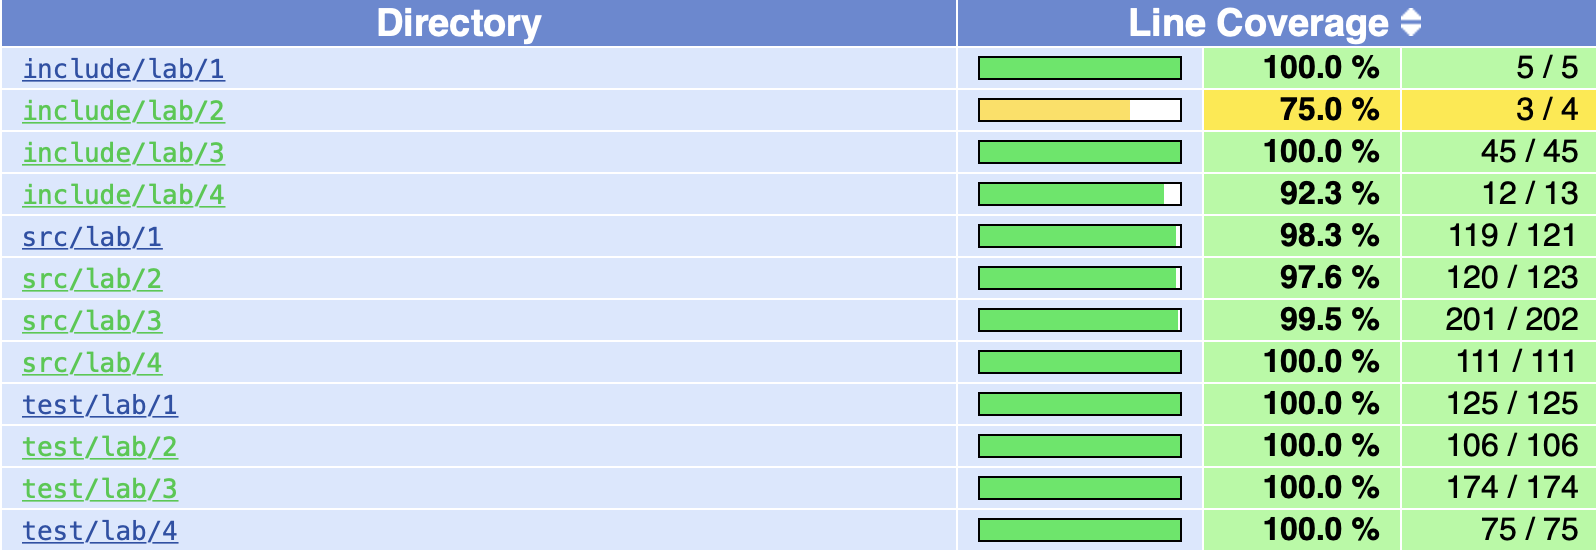
\includegraphics[scale=.5]{cov.png}
\end{figure}

\section{实验结果与分析}\label{sec:test24}
本次实验加深了对线性表的概念、基本运算的理解,
掌握了线性表的基本运算的实现。
深刻理解了线性表的\emph{逻辑结构}和\emph{物理结构}之间的关系。
并通过与实验一的对比,了解到了线性表不同的物理存储结构之间的相同点与不同点。
\par
作为第二次实验,本次实验的内容还是相对比较简单的,通过整个编程过程,我又熟悉了一遍链表的实现,对原先的知识进行了一次很好的复习。
\par 整个实验均在\texttt{UNIX}环境下编程
所有的代码均采用\emph{Google C/C++}标准代码规范,
通过\texttt{clang-format}和\texttt{clang-tidy}进行格式化和规范化。
\par
同时,在编码过程中,我尽可能地使用了更加现代化的C++代码,例如使用智能指针(\textit{unique\_ptr})来进行资源管理,从而避免了手动管理内存而可能带来的内存泄漏等问题、
例如使用\texttt{auto}关键字来声明函数与变量,从而减少了错误的类型声明或不正确的隐式类型转换。
使得代码可读性更高,更容易维护,更加健壮。这样的规范和编码习惯有助于以后在工作中更高效地完成工作任务。
\par
本系统完整的实现了课程要求的全部功能,并且实现了多线性表管理和文件存储功能,
系统健壮性良好,可以应对各种情况的输入,且能输出相应的错误提示。
系统测试覆盖度接近100\%,可以认为不会发生逻辑错误
\par


\backmatter

\begin{ack}
    感谢老师、助教和同学在本次实验中的对我的帮助,特别是许老师和助教许学长,在实验中为我提供了很多建议。
    \par
    在此衷心地对他们表示感谢!
    \par
    特别感谢教材\cite{严蔚敏2002数据结构}与习题册\cite{严蔚敏1998数据结构题集}对我的帮助
\end{ack}

\bibliography{book}

\appendix

\chapter{实验源代码}\label{appendix:1}
\section{文件结构}\label{appendix:structure}
\lstinputlisting{../tree.dat}
\section{实验一源代码}\label{appendix:lab1}
\subsection{线性表实现代码}
\emph{构造函数与初始化——List.cc}
\lstinputlisting[language=c++]{../src/lab/1/List.cc}
\emph{元素操作——elem.cc}
\lstinputlisting[language=c++]{../src/lab/1/elem.cc}
\emph{插入删除等操作——modify.cc}
\lstinputlisting[language=c++]{../src/lab/1/modify.cc}
\emph{文件操作——fs.cc}
\lstinputlisting[language=c++]{../src/lab/1/fs.cc}
\emph{CMake配置}
\lstinputlisting{../src/lab/1/CMakeLists.txt}
\subsection{测试代码}\label{appendix:test1}
\emph{构造函数与初始化测试——List\_test.cc}
\lstinputlisting[language=c++]{../test/lab/1/List_test.cc}
\emph{元素操作测试——elem\_test.cc}
\lstinputlisting[language=c++]{../test/lab/1/elem_test.cc}
\emph{插入删除等操作测试——modify\_test.cc}
\lstinputlisting[language=c++]{../test/lab/1/modify_test.cc}
\emph{文件操作测试——fs\_test.cc}
\lstinputlisting[language=c++]{../test/lab/1/fs_test.cc}

\section{实验二源代码}\label{appendix:lab2}
\subsection{线性表实现代码}
\emph{节点构造函数与初始化——Node.cc}
\lstinputlisting[language=c++]{../src/lab/2/Node.cc}
\emph{线性表构造函数与初始化——List.cc}
\lstinputlisting[language=c++]{../src/lab/2/List.cc}
\emph{元素操作——elem.cc}
\lstinputlisting[language=c++]{../src/lab/2/elem.cc}
\emph{插入删除等操作——modify.cc}
\lstinputlisting[language=c++]{../src/lab/2/modify.cc}
\emph{CMake配置}
\lstinputlisting{../src/lab/2/CMakeLists.txt}
\subsection{测试代码}\label{appendix:test2}
\emph{节点构造函数与初始化测试——Node\_test.cc}
\lstinputlisting[language=c++]{../test/lab/2/Node_test.cc}
\emph{线性表构造函数与初始化测试——List\_test.cc}
\lstinputlisting[language=c++]{../test/lab/2/List_test.cc}

\end{document}
\endinput
%%
